\clearpage
\chapter{Architektur}
(ES) In diesem Kapitel wird der technische Aufbau des Spiels beschrieben. Hierbei wird auf die verwendete Architektur sowie die zugrunde liegenden Designentscheidungen eingegangen.

\section{Einflussfaktoren für Architektur}
(ES) Die Maßgebenden Einflussfaktoren für die Entscheidung der verwendeten Softwarearchitektur, sind neben dem im Team vorhanden Know-How bezüglich Programmiersprachen und Unit-Tests, die eigenen Anforderungen an die optische Repräsentation des Spiels. Nach einer Aufnahme der Kenntnisse der Teammitglieder war schnell ersichtlich, dass die Programmiersprache Java am verbreitetsten ist und sich in Bezug auf Unit-Tests auch hier die größte Übereinstimmung findet.

Der in der Vorlesung zur Fallstudie vorgestellte Tomcat-Server bietet die Möglichkeit, für ein in Java geschriebenes Fachkonzept ein Userinterface auf HTML-Basis bereitzustellen. Da die in Java zur Verfügung stehende SWING-Bibliothek nicht die gewünschten optischen Resultate erzielt, wurde diese schnell ausgeschlossen.

\section{Übersicht über technischen Aufbau}
(ES) Aus den zuvor genannten Beweggründen ergab sich schnell der in \ref{fig:abb29} 
\begin{figure}[!h]
	\centering
	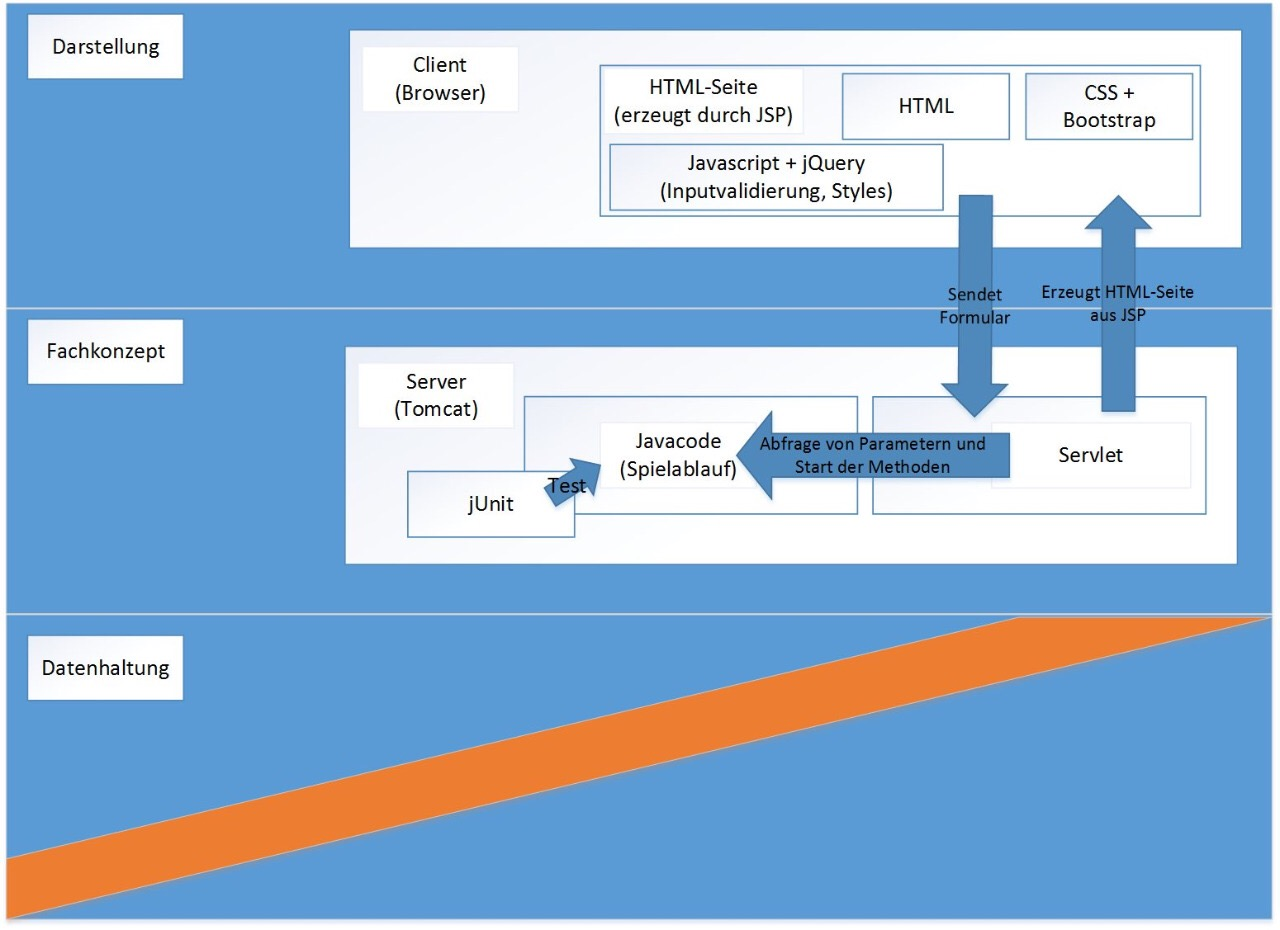
\includegraphics[scale=0.2]{img/3-schichten-modell.jpeg}
	\caption{3-Schichten-Modell} \label{fig:abb29}
\end{figure}
dargestellte Aufbau der Software. Im ersten Schritt zur Gliederung der Architektur wurde die aus dem Studium bekannte 3-Schichten-Architektur zugrunde gelegt. Die Software wird hierbei in die ebenen Datenhaltung, Fachkonzept sowie Darstellung untergliedert. Bei den vorgegebenen Anforderungen an die Fallstudie, ist eine Datenhaltung als optional angegeben. Zur Reduzierung des Programmieraufwandes wurde auf eine Datenbankanbindung oder sonstige Datenhaltung verzichtet.

Zur Umsetzung des Fachkonzeptes wird auf die Programmiersprache Java gesetzt. Wobei die gesamte Spiellogik so umgesetzt ist, dass hierauf ein beliebiges Userinterface aufgesetzt werden kann. Zum Testen des Fachkonzepts kommt JUnit zum Einsatz. Da als Userinterface eine Webseite dienen soll, wird das Fachkonzept nicht in einer lokalen JVM sondern auf einem Webserver ausgeführt. Der zum Einsatz kommende Tomcat-Server kann sowohl den Java-Code des Fachkonzepts ausführen, als auch über die gewünschte Webseite Eingaben des Anwenders entgegen nehmen, bzw. entsprechende Ausgaben zurückgeben. Die dabei zum Einsatz kommenden Techniken werden in den folgenden Kapiteln näher erläutert.

Bei der Darstellungsebene des Spiels werden die gestalterischen Möglichkeiten von HTML, CSS sowie JavaScript genutzt, indem der Tomcat-Server für den Anwender eine entsprechende Webseite als Userinterface zur Verfügung stellt. Die Bedienung des Spiels erfolgt somit für den Anwender in einem Webbrowser.

Folglich ergibt sich, neben einer logischen Trennung von Fachkonzept und Darstellung, eine technische Trennung, in Form einer Client-Server-Architektur. Auf dem Server wird die Spiellogik ausgeführt, eine dynamische Webseite generiert und auf Eingaben des Anwenders gewartet. Im Browser des Clients wird hingegen die dynamisch generierte Webseite mit den aktuellen Werten des Spielstandes angezeigt, als auch eine Eingabemöglichkeit zur Ausführung von gewünschten Spielaktionen geboten.

\section{Laufzeitumgebung}
(ES) Da die Spiellogik in Java programmiert ist, wird zur Ausführung des Programms eine Java-Laufzeitumgebung benötigt. Während der Entwicklung wird hier im speziellen die Java Runtime Environment in Version 8 verwendet. Eine weitere wichtige Komponente ist der Servlet-Container. Die an den Server übermittelten Eingaben, in Form von Http-Requests, werden vom Webserver entgegen genommen und an den Servlet-Container weitergeleitet. Dieser verarbeitet die Requests und leitet diese an das Servlet, welches im folgenen Kapitel näher beschrieben wird, weiter. Zur Bereitstellung einer serverseitigen Java-Laufzeitumgebung, als auch einem Servlet-Container, dient der bereits angesprochene Tomcat-Server von Apache.

\section{Java Servlets}\label{sec:Servlets}
Auf dem bereits erwähnten Tomcat-Server wird eine Instanz der Klasse Servlet ausgeführt. Hierüber wird es ermöglicht, auf Eingaben des Anwenders zu reagieren und entsprechende Rückgaben auszuliefern. Die Kommunikation zwischen Server und Client erfolgt hierbei mittels Http-Requests. In diesem Fall wird die doPost()-Methode der Klasse HttpServlet überschrieben und mit den gewünschten Funktionalitäten versehen.

Der Aufruf der Methode erfolgt von Seiten des Clients durch absenden eines HTML-Formulars. Im Kapitel \ref{UI} auf Seite \pageref{UI} wird hier näher drauf eingegangen. Innerhalb der doPost()-Methode können über das request-Objekt auf die vom Anwender getätigten Eingabeparameter zugegriffen werden. Aufgrund der Eingaben des Anwenders werden die entsprechenden Methoden der Spiellogik mit den benötigten Übergabeparametern aufgerufen. Bei einem ggf. stattzufindenden Seitenwechsel im Browser werden weiterhin entsprechende Übergabeparameter dem request-Objekt hinzugefügt und die neue Seite unter Mitgabe des Objekts aufgerufen.

Zur weiteren Vereinfachung des Programmieraufwandes wird innerhalb der Servlet-Instanz nicht nur die Kommunikation mit dem Client koordiniert, sondern auch eine Instanz des Spiels erzeugt. Alle innerhalb der doPost()-Methode getätigten aufrufe bezüglich der Spiellogik werden somit an die Instanz des Spiels übergeben. Auch wenn auf abstrakter Ebene das Servlet und die Spiellogik als zwei getrennte Elemente betrachten werden, ist die Spielinstanz real gesehen eine Instanz innerhalb des Servlets.

\section{JavaServer Page}
(ES) Wie im Kapitel \ref{sec:Servlets} auf Seite \pageref{sec:Servlets} beschriebenen werden in der doPost()-Methode neue Webseiten unter Mitgabe des request-Objekts aufgerufen. Da eine nur mit HTML erstellte Seite mit dem request-Objekt nicht umgehen kann, kommt zur Erstellung der Webseite JavaServer Page bzw. Expression Language zum Einsatz. Der Einsatz beider beschränkt sich jedoch innerhalb dieses Projektes auf die Angabe des Ziels des HTML-Formulars sowie als Platzhalter für Variablen zur dynamischen Erstellung von Seiteninhalten.

Die Webseite wird wie gewohnt mit HTML erstellt, wobei die dynamisch zu erstellenden Inhalte im Quellcode durch Value Expressions ( \$\{ Value \} ) ersetzt werden. Beim Aufruf der Seite innerhalb der doPost()-Methode werden die Value Expressions mit den gleichnamigen Parametern aus dem request-Objekt ersetzt und der so entstehende HTML-Code an den Browser des Clients ausgeliefert. In diesem Projekt werden hierdurch vor allem Textinhalte innerhalb von HTML-Elementen generiert bzw. bestimmte Werte dem Class-Attribut der HTML-Elemente hinzugefügt.

\section{User Interface}\label{UI}
(ES) Zur Erstellung des Userinterface kommen überwiegend die für Webanwendungen üblichen Technologien in Form von HTML5, CSS3 und JavaScript sowie aktuell gängige Frameworks zum Einsatz. Die logische Strukturierung der Seiten erfolgt mittels der Auszeichnungsprache HTML. Die Gestaltung des Userinterface in Bezug auf Layout, \enquote{Look and Feel} erfolgt überwiegend mittels CSS3 sowie zur Reduzierung des Programmieraufwands mittels dem CSS-Framework Bootstrap. JavaScript sowie das JS-Framework jQuery werden zur logischen Validierung von Benutzereingaben siwue zur Umsetzung einiger kontextbezogener optischer Effekte bzw. Layoutumgestaltungen, welche sich mittels CSS schwierig oder nicht umsetzten lassen.

Die Aufteilung des Userinterface auf mehrere JSP-Dokumente ergibt sich in erster Linie aus an den Server zu schickenden Formularen und dem im Servlet definierten Requests. Für jedes zu versendende Formular wird ein eigenes JSP-Dokument verwendet. Die Formulare wiederum repräsentieren logische Spielabschnitte.

Die Startseite beinhaltet eine Auswahlmöglichkeit für die gewünschte Spieleranzahl sowie einen Button zum Start des Spiels. Mit Klick auf den Start-Button wird das Formular an das Servlet gesendet. Es wird das Spiel-Objekt mit der ausgewählten Anzahl an Spielern erzeugt und anschließend die erste Spielrunde mit dem ersten Spielzug des ersten Spielers begonnen.

In der ersten Spielrunde eines jeden Spielers wird dieser auf eine weitere Seite geführt. Hier hat der Spieler zu entscheiden auf welche Sparte bzw. welches Marktsegment sein Unternehmen zu Beginn ausgerichtet ist. Mit Versandt des Formulars an den Server erfogt in der doPost()-Methode eine Abfrage welcher Button dsa Formular versendet hat, genauer gesagt, welcher Button zum aktuellen Zeitpunkt einen Value dem Http-Request mitgegeben hat. Dementsprechend erfolgt die Ausführung der entsprechenden Methoden im Fachwerk zum Freischalten der ausgewählten Sparte beim jeweiligen Spieler und Erzeugung der ersten Uhr für das ausgewählte Marktsegment. Der letzte Schritt in diesem Abschnitt ist dann die Weiterleitung des Spielers an die für ihn benötigten Auswahl- wowie Anzeigeelemente für eine Spielrunde.

Aufgrund des Quellcodeumfangs zur Darstellung der Eingabemaske, für die vom Spieler während eines Spielzugs zu tätigenden Aktionen, bzw. zur Anzeige seiner aktuellen Spielinformationen, ist der entsprechende Quellcode auf mehrere Dateien aufgeteilt. Eine Datei beinhaltet die Navigationselemente sowie das \enquote{Grundgerüst} der Seite. Die durch die Navigationselemente umschaltbare Spielelemente sind zur besseren Übersicht über den Quellcode in weitere Dateien ausgelagert. JSP bietet hier die Möglichkeit die ausgelagerten Dateien mittels jsp:include einzubinden. Während der serverteitigen Kompilierung werden aus den einzelnen Dokumenten ein einzelnes Dokument für den Client bzw. dessen Browser erstellt. 

Mittels Buttons kann der Spieler wählen, welche Aktionen in der aktuellen Spielrunde durchgeführt werden sollen. Ein Script, mittels JavaScript umgesetzt, übergibt an das jeweilige versteckte Inputfeld einen entsprechenden Wert.
Nach Tätigung aller während der aktuellen Spielrunde gewünschten Spielaktionen, kann der Spieler den Button \enquote{Runde beenden} betätigen. Die in den versteckten Inputfeldern gesammelten Spielaktionen werdenüber das HTML-Formular in Form eines Http-Requests an die doPost()-Methode innerhalb des Servlet-Objekts weitergeleitet. Innerhalb der Methode wird geprüft welche Buttons angeklickt wurden und die äquivalenten Methoden im Fachkonzept ausgeführt sowie die Methode zum Wechsel des Spielers aufgerufen. Am Ende dieses Abschnittes wird eine neue Seite mit Anzeige der aktuellen Runde sowie des nächsten Spielers angezeigt. Dieser kann gemäß des Hot-Seat-Verfahrens den Platz am Bildschirm einnehmen und seine Runde beginnen. Zum Ende der letzen Spielrunde wird das letzte Dokument zur Darstellung des Gewinners, bzw. der Gewinnreihenfolge der Spieler angezeigt. Unterhalb der Gewinneranzeige gibt es die Möglichkeit ein neues Spiel zu starten.

Neben der Dokumentenstruktur ist die Verwendung von CSS-Regeln und CSS-Klassen ein weiteres wichtiges Element der Umsetzung des Userinterface. Die CSS-Regeln sind derart gestaltet, dass je nachdem was der Spieler freigeschalten bzw. nicht freigeschaltenen hat, eine entsprechende optische Darstellung erfolgt. Als Selektoren kommen hierbei überwiegend CSS-Klassen zum Einsatz. In den entsprechenden HTML-Elementen sind im Value-Bereich des class-Attributs Value Expressions eingebettet. Je nach freigeschaltenen Spielelementen werden im request-Objekt entsprechende Werte hinterlegt. Beim Kompilieren der Webseite werden die Value Expressions ggf. durch die entsprechenden Werte im request-Objekt ersetzt und somit die definierte CSS-Klasse beim HTML-Element definiert. Im Spielerobjekt hinterlegte Werte wie zum Beispiel das aktuelle Kapital oder der Warenbestand der Uhren werden auf die gleiche Art und Weise der Webseite übergeben. Die Value Expressions sind dann jedoch so im Quellcode plaziert, dass diese als Text ausgegeben werden und nicht dem jeweiligen Element als class-Atribute mitgegeben werden.

\lstset{language=HTML}
\begin{lstlisting} [caption={Geschriebener Quellcode mit JSP},label=JSP-Code,captionpos=b]
<div id="watch0" class="card ${watch0}">
<h4>Modell 1</h4>
<p>Produktlinie: ${m0s}</p>
\end{lstlisting}

\lstset{language=HTML}
\begin{lstlisting} [caption={Kompilierter HTML-Code},label=compiled-HTML,captionpos=b]
<div id="watch0" class="card card-aktive">
<h4>Modell 1</h4>
<p>Produktlinie: Umwelt</p>
\end{lstlisting} 

\section{Eingabeüberprüfung im UI durch JavaScript}
(EA) Da der Java-Code nicht im im HTML-basierten UI abgebildet ist benötigt es auf UI-Ebene eine weitere Logik. Diese ist notwendig, um die vom Benutzer getätigten Eingaben zu überprüfen und somit keine ungültigen Werte an das Spiel zu übergeben. 

\subsection*{Kontostand prüfen}

\lstset{language=Java}
\begin{lstlisting} [caption={Überprüfung Kontostand},captionpos=b]
function getMoney()
{
return parseFloat($('#money').text().replace(/[\.\u20ac]/g,''));
}
\end{lstlisting}

(EA) Jedes mal wenn eine Aktion ausgeführt werden soll, die Geld kostet, wird zuerst der Kontostand überprüft bevor sie ausgeführt wird. Die Aktionen eines Buttons werden über das \enquote{onclick-Event} abgefangen. Damit diese jedoch nicht nicht immer ausführbar ist wird in die \enquote{onclick} Eigenschaft des Buttons eine Bedingung eingefügt. 

\lstset{language=HTML}
\begin{lstlisting} [caption={OnClick-Event mit Bedingung für Kontostandüberprüfung},captionpos=b]
<li class="${clOc1} list-group-item">Holz 
<span class="glyphicon glyphicon-ok"></span>
<a class="addBtn" onclick="if(getMoney() >= $(this).text().replace(/[\.\+\u20ac]/g,'')  && !$(this).hasClass('d')){research('researchCaseOeko',1); change($(this)); }else if($(this).hasClass('d')){research('researchCaseOeko',1); change($(this));}else{notEnough()}">+ ${clCOc1} &euro;</a>
</li>
\end{lstlisting}

(EA) In dieser Bedingung wird geprüft, ob die Kosten der Aktion durch den aktuellen Kontostand gedeckt sind. Ergibt diese Prüfung \enquote{true}, so wird die jeweilige Aktion ausgeführt, es erfolgt eine Meldung auf dem Bildschirm, der Button ändert seine Beschriftung und die jeweiligen Kosten werden direkt vom Konto abgezogen.

\begin{figure} [H]
	\centering
	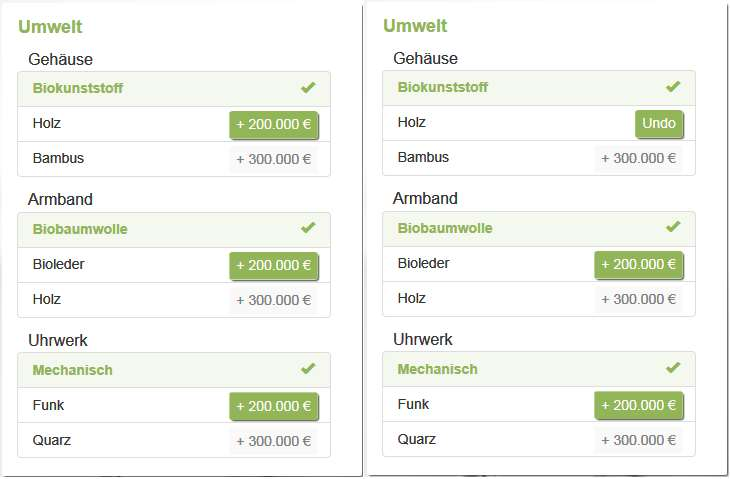
\includegraphics[scale=0.38]{img/button-do-undo.jpeg} 
	\caption{Button: do-undo} \label{fig:abb30}
\end{figure}

Beim erneuten Drücken auf den Button wird der Kontostand wieder um den vorher abgezogenen Betrag erhöht und die Kosten für die Aktion werden wieder auf dem Button ausgewiesen. 

Wenn der Kontostand jedoch nicht ausreicht und der Button auch nichts bereits einmal gedrückt wurde, so wird die Funktion \enquote{notEnough()} ausgeführt, welche eine Meldung auf dem Bildschirm ausgibt, dass das Geld nicht ausreicht. 

\lstset{language=Java}
\begin{lstlisting} [caption={Ausgabe bei zu geringem Kapital},captionpos=b]
function notEnough()
{
alert('Das Kontoguthaben reicht nicht aus!');
}
\end{lstlisting}

Folglich wird die Aktion des Buttons auch nicht ausgeführt.

\subsection*{Eingabeüberprüfung in den Abteilungen}

(EA) In den diversen Abteilungen müssen verschiedene Eingabemöglichkeiten berücksichtigt werden. 

\subsection*{Forschung \& Entwicklung}

(EA) Hier ist es nur möglich Erweiterung für das jeweilige Segment freizuschalten, wenn das Kontoguthaben ausreicht. Des Weiteren ist es auch nur möglich ein neues Segment freizuschalten, wenn ebenfalls das Geld ausreicht.

Es wird aber auch ein bereits bestehender Bestand berücksichtigt, da Produktveränderungen auch an vorhandenen Uhren durchgeführt werden müssen. Dies verursacht somit einen zusätzlichen Aufwand. 

\subsection*{Produktion}

\lstset{language=Java}
\begin{lstlisting} [caption={Eingabeüberprüfung Produktion},captionpos=b]
$('#output0').blur(function()
{
if($(this).val())
{
if($(this).hasClass('d'))
{
let undoProdCost = $(this).attr('class').replace('d','').replace('numInput','');
let undoSum = getMoney() + undoProdCost * parseFloat($('#ekVal0').text().replace(/[\.\u20ac]/g,''));
$('#money').text(undoSum.toLocaleString('de-DE',{minimumFractionDigits: 2}));

if($(this).val() > parseInt($('#productionLimit0').text().replace(/[\.]/g,'')))
{
alert("Die Produktionskapazitaeten reichen nicht aus!\nDas Limit betraegt: "+$('#productionLimit0').text());
$(this).attr('class','numInput');
$(this).val('');
}
else
{
if(getMoney() >= ($(this).val() * parseFloat($('#ekVal0').text().replace(/[\.\u20ac]/g,''))))
{
let prodCost = $(this).val() * parseFloat($('#ekVal0').text().replace(/[\.\u20ac]/g,''));
let difference = getMoney() - prodCost;
$('#money').text(difference.toLocaleString('de-DE',{minimumFractionDigits: 2}));
$(this).attr('class','numInput');
$(this).addClass('d');
$(this).addClass($(this).val());
}
else
{
alert("Das Guthaben reicht nicht aus!");
$(this).val('');
$('#prodCost0').val('');
}
}
}
else
{
if($(this).val() > parseInt($('#productionLimit0').text().replace(/[\.]/g,'')))
{
alert("Die Produktionskapazitaeten reichen nicht aus!\nDas Limit betraegt: "+$('#productionLimit0').text());
$(this).val('');
$('#prodCost0').val('');
}
else
{
if(getMoney() >= ($(this).val() * parseFloat($('#ekVal0').text().replace(/[\.\u20ac]/g,''))))
{
let prodCost = $(this).val() * parseFloat($('#ekVal0').text().replace(/[\.\u20ac]/g,''));
let difference = getMoney() - prodCost;
$('#money').text(difference.toLocaleString('de-DE',{minimumFractionDigits: 2}));
$(this).addClass('d');
$(this).addClass($(this).val());
}
else
{
alert("Das Guthaben reicht nicht aus!");
$(this).val('');
$('#prodCost0').val('');
}
}
}
}
else if(!$(this).val())
{
if($(this).hasClass('d'))
{
let undoProdCost = $(this).attr('class').replace('d','').replace('numInput','');
let undoSum = getMoney() + undoProdCost * parseFloat($('#ekVal0').text().replace(/[\.\u20ac]/g,''));
$('#money').text(undoSum.toLocaleString('de-DE',{minimumFractionDigits: 2}));
$(this).attr('class','numInput');
}
}
});

\end{lstlisting}

(EA) In der Abteilung Produktion lässt sich die Menge der zu produzierenden Uhren angeben. Die Menge ist jedoch durch die Produktionskapazität begrenzt. Insofern wird auf Eingaben, welche die Kapazität übersteigen durch eine Meldung hingewiesen und das Eingabefeld wird geleert. 

Wenn die Produktionsmenge jedoch im Rahmen des Möglichen liegt, so wird überprüft ob das Guthaben zu dem Zeitpunkt für die geplante Menge ausreicht. Ansonsten erfolgt die Meldung, dass dies nicht der Fall ist. 

Dadurch dass das Geld sofort nach der Eingabe abgezogen wird muss berücksichtigt werden, dass Eingaben wieder rückgängig gemacht werden können. Insofern wird erkannt dass bereits eine Eingabe erfolgt ist und bei Änderung werden die vorher abgezogenen Beträge erst wieder auf das Konto hinzu addiert um danach die neuen Produktionskosten abziehen.

\subsection*{Einkauf}

(EA) Beim Einkauf gibt es die Möglichkeit Produktressourcen durch Verbesserungen billiger zu beziehen. Hierbei erfolgt auch die Prüfung ob das Guthaben ausreicht.

\subsection*{Vertrieb}

(EA) Im Vertrieb wird lediglich überprüft der Verkaufspreis mit der geplanten Absatzmenge multipliziert. Wobei auch die Absatzmenge durch den Vorrat begrenzt ist.

\lstset{language=Java}
\begin{lstlisting} [caption={Eingabeüberprüfung Vetrieb},captionpos=b]
$('#quantitySupplied0').blur(function()
{
if( !$(this).val() == '')
{
if(!$('#offerPrice0').val() == '')
{
if($(this).val() > parseInt($('#stock0').text().replace(/[\.]/g,'')))
{
alert('Der Vorrat reicht nicht aus! \nVorrat: '+$('#stock0').text());
$(this).val('');
}
else if($(this).val() > 0 && $(this).val() <= parseInt($('#stock0').text().replace(/[\.]/g,'')))
{
alert($(this).val().toLocaleString('de-DE',{minimumFractionDigits: 2}));
alert($('#offerPrice0').val());
let verkauf = parseFloat($(this).val().toLocaleString('de-DE',{minimumFractionDigits: 2})) * parseFloat($('#offerPrice0').val());
$('#verkauf0').text(parseFloat(verkauf)+ ' \u20ac');
}
}
else
{
alert('Sie m\u00fcssen zuerst einen Verkaufspreis eingeben!');
$(this).val('');
}
}
});
\end{lstlisting}

\clearpage
\chapter{Entwickungsumgebung}
\section{Eclipse JAVA EE IDE}
(NF) Eclipse ist eine Programmierumgebung als Entwicklungswerkzeug von Software und Programmen aller Art. Es gibt eine Vielzahl von kommerziellen und kostenlosen Erweiterungen. Unter Eclipse ist es möglich nahezu jede Programmiersprache zu entwickeln. Für das Projekt wurde lediglich die Programmiersprache Java für die Logik der Simulation verwendet. Als integrierte Entwicklungsumgebung umfasst Eclipse nicht nur einen Texteditor zum erstellen des Quellcodes, sondern viele weiterere für die Softwareentwicklung benötigten oder hilfreichen Programme bzw. Funktionen. Diese lassen sich dank des modularen Aufbaus von Eclipse in beliebiger Kombination hinzufügen, oder man verwendet eine der für bestimmte Anwendungsfälle bereits vorkonfigurierten Versionen. Aufgrund der Verwendung einer Server-Client-Architektur unter Verwendung von Java Servlets, bietet es sich an, die entsprechende Version Eclipse JAVA EE IDE zu verwenden. Diese Version beinhaltet gleich die benötigten Komponenten, um den Tomcat-Server in die IDE einbinden zu können. Das Testen einzelner Funktionen kann somit innerhalb der Entwicklungsumgebung erfolgen und eine separate Verwaltung eines Webservers zu Testzwecken ist somit nicht erforderlich.
\section{Git}
(NF) Bei Git handelt es sich um eine freie Software zur Versionsverwaltung. Git ist Open Source und lediglich per Kommandozeile verfügbar. Dennoch gibt es bereits unzählige grafische UIs, die Git vereinfachen und seine Befehle grafisch darstellen (beispielhaft dafür: Sourcetree, GitHub Desktop oder TortoiseGit) . Git wird auch von zahlreichen Großprojekten verwendet, darunter Android, LibreOffice oder jQuery. 
\section{GitHub}
(NF) GitHub ist der webbasierte Online-Dienst, welcher Entwicklungsprojekte auf einem Server bereitstellt und somit Filehosting betreibt. Grundsätzlich ist es nicht anderes als Git, eben nur nicht lokal, zudem bringt GitHub seinen eigenen grafischen UI Client namens GitHub Desktop mit. Ein grafischer Client wurde in diesem Projekt nicht mitgliederübergreifend eingesetzt. Weiterhin bieten viele Entwicklungsumgebungen wie auch Eclipse eine integrierte Möglichkeit auf die gehosteten Softwarerepositories zuzugreifen. Auch diese Lösung kam im Team zum Teil in Einsatz.
\section{LaTeX}
(NF) Für die Erstellung der Dokumentation wurde das Softwarepaket LaTeX genutzt. Als Editor wurden überwiegend TeXstudio oder der zur Softwareentwicklung gedachte Texteditor Atom eingesetzt.\\
LaTeX ist ein Softwarepaket, welches die Benutzung des Textsatzsystems TeX mit Hilfe von Makros vereinfacht.
LaTeX ist die populärste Methode TeX zu verwenden.
TeXstudio ist ein plattformunabhängiger Editor zur Erstellung von genannten LaTeX Dokumenten.\\
Beide sind Open-Source und kostenlos. Neben TeXstudio gibt es noch eine Vielzahl an weiteren Editoren, speziell für LaTeX Dokumente.

